% Group: 	2
% Name: 	Coding Pharaohs
% Document: 	SDD incomplete first draft
% Author:	Matthew Nestor
% Date:		Tuesday September 10 2013

\documentclass[11pt, a4paper,titlepage]{article}
\usepackage{acronym}
\usepackage[pdftex]{graphicx}
\usepackage{float}
\topmargin -1cm

\begin{document}
\begin{titlepage}
\centerline{\small The University of Adelaide}
\centerline{\small COMP SCI 3006/7015 Software Engineering and Project}
\vspace{5cm}
\centerline{\bf \huge Software Design Document}
\centerline{\bf \huge (SDD)}
\vspace{0.5cm}
\centerline{\LARGE for}
\vspace{0.5cm}
\centerline{\bf \huge Road Closure Marking}
\centerline{\bf \huge Robot (prototype)}
\vspace{1cm}
\centerline{Version 0.3}
\vspace{1cm}
\centerline{Prepared by Group 2}
\end{titlepage}

\tableofcontents
%\pagebreak
%\listoffigures
%\pagebreak
%\listoftables

\newpage
{\bf \large Change History}\newline

\begin{tabular}{| c | c | l |}
\hline
Date & Version & Reason for Change \\
\hline
10th Sept & 0.1 & Initial draft \\
\hline
15th Sept & 0.2 & Expanded sections 2,3,4 \\
\hline
19th Sept & 0.3 & Expanded sections 7,8 and minor changes \\
\hline
\end{tabular}

\newpage

\section{Introduction}

\subsection{Purpose}

SDD, which is abbreviation for Software Design Document, describes the implementation procedures of a software project. Specifically, it is needed to transfer a specification into an executable system. This document is the SDD for developing a robot to mark road closures in a city, which is destroyed by a natural disaster. \\
\\
This SDD will document the GUI, AI, Robot Move, Map Representation, and Communication that will be utilized in implementing the system for the robot. \\

\subsection{Scope}
The aim of this project is to develop a prototype of a robot which may be used to produce a map of the ruined city and mark the road closures in order to prevent people from moving into these areas. \\
\\
The map includes virtual representations of the closures, disaster area, the obstacles, the intersection and roads, and unexplored areas which includes anything I mentioned above. And the physical map includes using cardboard or some rigid material to represent obstacles and put them randomly, and using black lines as roads. The most important is that the robot should detect the disaster area and mark the road closures with a whiteboard marker. And in this procedure, the robot also has to avoid the obstacles and go forward. \\
\\
The virtual map will be dynamically displayed on the system’s Graphical User Interface (GUI), and it is created and exported in the form of an Extensible Markup Language (XML) document. \\
\\
Within the map, the robot will move from the start point and explore the whole map so that it can identify where the obstacles are and mark where the road closures are. \\
\\
For the purposes of this project the city is no larger than A1 paper size. \\

\subsection{Related Documents}

This SDD should be related to the other project documents, namely the Software Project Management Plan (SPMP), the Software Requirement Specification (SRS). \\

\subsection{Overview}

This SDD consists of the following:

\begin{itemize}
\item Introduction introduces the aims and function of the project;
\item System Overview briefly gives a broad outline of the architecture of the project;
\item System Architecture and Components Design gives a detailed description of the
 project architecture, including its composite components;
\item Data Design describes the a variety of data structures used in the project;
\item Design Details includes the Class, State and Interaction Diagrams in this project;
\item Human Interface Design describes the perspective of the
 user to utilize the robot. 
\item  Resource Estimates summaries computer resource estimates required for operating
 the robot.
\end{itemize}

\subsection{Document Conventions}

All diagrams unless otherwise noted follow standard UML conventions. 

\section{System Overview}

\subsection{Background}

The Road Closure Marking Robot is a prototype of an on-road, land-vehicle style robot, whose function is to investigate disaster-stricken urban zones and mark road closures to prevent access to hazardous areas. As this model is a prototype, the robot is miniaturised, and rather than following city roads, it follows black lines on an A1 size sheet of paper. \\
\\
For a full description of the requirements, see the accompanying SRS. \\
  
\subsection{Technologies Used}

The LEGO Mindstorms NXT robot set was used to create the prototype, as its size and sensor functionality make it well suited as a prototype. Items used from the NXT set include the intelligent brick, three servo motors, an ultrasonic sensor, a light sensor, two touch sensors, two large wheels, one small wheel, and various connecting parts. The Intelligent brick is the computer and controller for the robot's motors and sensors. The brick has been flashed with leJOS firmware. LeJOS is a Java extension for the programming of the LEGO Minstorms NXT. Thus, all software for the project shall be written in Java and leJOS. \\
\\
The host system and intelligent brick communicate via bluetooth. \\
  
\subsection{Software Design Overview}

The system consists of two sides: the robot side and the host side. The robot side is run on the NXT intelligent brick, and the host side is run on a remote terminal. The two sides communicate via bluetooth. The robot has two modes: automatic and manual. In automatic mode, the robot uses artificial intelligence to navigate to disaster zones and mark road closures on its own. In manual mode, a user controls the robot via a graphical display on the host side. The robot has the ability to create, save, and load maps of city areas. The maps contain information about such things as the city roads, disaster zones, the robot's location, and explored and unexplored areas (for more detail see section 4). The maps are represented graphically to the user on the host side, but are also available to the AI, and are used to efficiently guide the robot to roads in need of closure. \\

\section{System Architecture and Components Design}

\subsection{Architectural Description}

\begin{figure}[h]
\centering
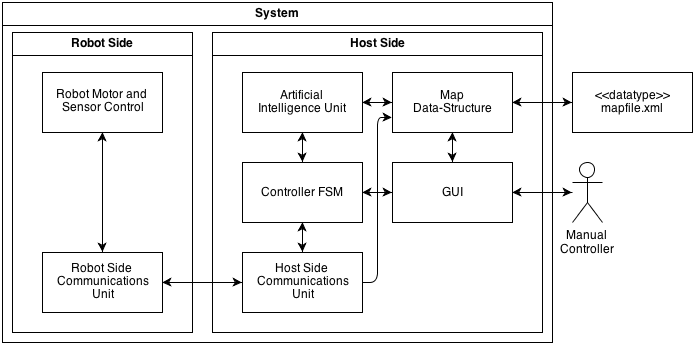
\includegraphics[width=15cm]{SystemArchitectureOverview2.png}
\caption{A graphical display of the system architecture}
\label{Figure 1}
\end{figure}

\noindent The system employs a pipe-and-filter architectural pattern, and consists of a Robot Side and a Host Side (see figure 1). \\
\\
The robot side contains the following subsystems:

\begin{itemize}
\item {\bf Robot Motor and Sensor Control:} Responsible for parsing movement commands from the Robot Side Communications Unit and turning them into leJOS motor commands. Responsible for receiving sensor data from the robot and sending it to the Robot Side Communications Unit. Responsible for initiating emergency stop under certain circumstances (e.g. bluetooth connection failure).
\item {\bf Robot Side Communications Unit:} Responsible for receiving sensor data from Robot Motor and Sensor Control, and passing that data via bluetooth to the Host Side Communications Unit. Responsible for receiving movement commands from the Host Side Communications Unit via bluetooth, and passing them to Robot Motor and Sensor Control. Responsible for sending a ``stop'' message to Robot Motor and Sensor Control in the event of a bluetooth connection failure.
\end{itemize}

\noindent The Host Side uses the Manager Model, a centralised control style architecture. It contains the following subsystems:

\begin{itemize}
\item {\bf Host Side Communications Unit:} Responsible for receiving sensor data from the Robot Side Communications Unit via bluetooth, and passing it to the Controller FSM. Responsible for receiving commands from the Controller FSM and sending them to the Robot Side Communications Unit via bluetooth. Responsible for sending sensor data to Map Data-Structure for the purposes of updating the representation of the robot's location.
\item {\bf Controller FSM:} A finite state machine with two states: automatic and manual. It is responsible for intercepting and responding to events from the GUI, the Robot (via the communications units), and the Artificial Intelligence Unit.
\item {\bf Artificial Intelligence Unit:} A finite state machine with five states: initial, search, explore, mark, and return. It is responsible for the behaviour of the robot when the Controller FSM is in automatic mode.
\item {\bf Map Data-Structure:} Responsible for creating a map data-structure to be used by (1) the Artificial Intelligence Unit for the purposes of AI navigation, and (2) the GUI for the purposes of generating a graphical display of the map to the user. The data-structure can be loaded from, and saved to, an xml map file (see section 4 for details). Receives and interprets sensor data from the Host Side Communications Unit in order to update its representation of the robot's location.
\item {\bf GUI:} The graphical user interface for controlling the robot and representing to the user the current state of the robot and the city (for details see section 5). Also responsible for sending commands to the Controller FSM and for interpreting map and robot data from Map Data-Structure.
\end{itemize}
    
\subsection{Component Decomposition Description}
    
The following is an object oriented component decomposition description of the above subsystems: \\

\subsubsection{Robot Motor and Sensor Control}

The Robot Motor and Sensor Control subsystem consists of two components:

\begin {itemize}
\item SensorInfo
\item RobotBehaviourControl
\end {itemize}
    
\subsubsection{Robot Side Communications Unit}

The Robot Side Communications Unit consists of two components:

\begin{itemize}
\item RobotCommunication
\item BTReceiver
\end{itemize}
    
\subsubsection{Host Side Communications Unit}

The Host Side Communications Unit consists of two components.

\begin{itemize}
\item PCReceiver
\item PCComms
\end{itemize}

\subsubsection{Controller FSM}

Controller FSM contains only one component:

\begin{itemize}
\item ControllerFSM
\end{itemize}

\subsubsection{Artificial Intelligence Unit}

The Artificial Intelligence Unit consists of six components:

\begin{itemize}
\item Node
\item Edge
\item SearchTree
\item Pathfinder
\item Explorer
\item AiFsm
\end{itemize}
    
\subsubsection{Map Data-Structure}

The Map Data-Structure has only one component:

\begin{itemize}
\item Map
\end{itemize}

\subsubsection{GUI}
The GUI consists of two components:
\begin{itemize}
\item GuiOfSEP
\item MapDraw
\end{itemize}
    
\subsection{Detailed Components Design Description}

\subsubsection{SensorInfo}

\begin{itemize}
\item Component Identifier: SensorInfo
\item Purpose: To fulfil requirements R02, SRS section 3.1.2, R03, section 3.1.3, R04, section 3.1.4, R05, section 3.1.5, R06, section 3.1.6, and R07, section 3.1.7
\item Function: Responsible for constructing and the NXT sensor classes and providing convenience methodsmfor them.
\item Subordinates: None
\item Dependencies: RobotBehaviourControl
\item Interfaces: None
\item Data: Light sensor data, touch sensor data, ultrasonic sensor data, tachometer data
\end{itemize}

\subsubsection{RobotBehaviourControl}

\begin{itemize}
\item Component Identifier: RobotBehaviourControl
\item Purpose: To fulfil requirements R01, SRS section 3.1.1, R02, SRS section 3.1.2, R03, section 3.1.3, R04, section 3.1.4, R05, section 3.1.5, R06, section 3.1.6, and R07, section 3.1.7
\item Function: Creates an instance of SensorInfo. Receives commands from the Robot Side Communications Unit and turns them into leJOS motor commands. Retrieves sensor data from SensorInfo and sends it to the Host Side Communications Unit.
\item Subordinates: SensorInfo
\item Dependencies: RobotCommunication
\item Interfaces: None
\item Data: Motor command data
\end{itemize}
    
\subsubsection{RobotCommunication}

\begin{itemize}
\item Component Identifier: RobotCommunication
\item Purpose: To fulfil requirement R08, SRS section 3.1.8, and H05, SRS section 3.3.5
\item Function: Creates an instance of RobotBehaviourControl. Contains methods for opening and closing the connection between robot and host systems, creating datastreams between them, receiving commands from the Host Side Communications Unit, issuing commands to RobotBehaviourControl, and sending data to the Host Side Communications Unit. Responsible for sending a ``stop'' message to RobotBehaviourControl in the event of a bluetooth connection failure.
\item Subordinates: RobotBehaviourControl
\item Dependencies: PCComms
\item Interfaces: None
\item Data: motor command data, sensor data
\end{itemize}
    
\subsubsection{BTReceiver}

\begin{itemize}
\item Component Identifier: BTReceiver
\item Purpose: To fulfil requirement R08, SRS section 3.1.8, and H05, SRS section 3.3.5
\item Function: The main program which creates an instance of RobotCommunication and calls its connection setup
\item Subordinates: RobotCommunication
\item Dependencies: None
\item Interfaces: None
\item Data: None
\end{itemize}
    
\subsubsection{PCReceiver}

\begin{itemize}
\item Component Identifier: PCReceiver
\item Purpose: To fulfil requirement R08, SRS section 3.1.8, and H05, SRS section 3.3.5
\item Function: Interprets raw data received from RobotCommunication into light sensor, battery, tachometer, distance, and touch data. Contains convenience methods for retrieving interpreted data for each of the above sensors.
\item Subordinates: None
\item Dependencies: PCComms
\item Interfaces: None
\item Data: Sensor data
\end{itemize}
    
\subsubsection{PCComms}
    
\begin{itemize}
\item Component Identifier: PCComms
\item Purpose: To fulfil requirement R08, SRS section 3.1.8, and H05, SRS section 3.3.5
\item Function: Creates an instance of PCReceiver. Contains methods for opening and closing the connection between the robot and host systems. Passes raw data received from RobotCommunication to PCReceiver.
\item Subordinates: PCReceiver
\item Dependencies: RobotCommunication
\item Interfaces: None
\item Data: Motor command data, sensor data
\end{itemize}
    
\subsubsection{ControllerFSM}
    
\begin{itemize}
\item Component Identifier: ControllerFSM
\item Purpose: To fulfil system features, SRS section 4.1 and 4.2, and to fulfil system requirements H02, SRS section 3.3.2, and R09, section 3.1.9
\item Function: A finite state machine with two states: automatic and manual. It is responsible for intercepting and responding to events from the GUI, the Robot (via the communications units), and the Artificial Intelligence Unit.
\item Subordinates: AiFsm, GuiOfSEP
\item Dependencies: PCComms, AiFsm, GuiOfSEP
\item Interfaces: None
\item Data: Motor command data, sensor data, state data
\end{itemize}
    
\subsubsection{Node}
    
\begin{itemize}
\item Component Identifier: Node
\item Purpose: To fulfil requirements R09, SRS section 3.1.9, R01, section 3.1.1, and M01, section 3.2.1
\item Function: The node component of the SearchTree data-structure.
\item Subordinates: None
\item Dependencies: SearchTree
\item Interfaces: None
\item Data: None
\end{itemize}
    
\subsubsection{Edge}
    
\begin{itemize}
\item Component Identifier: Edge
\item Purpose: To fulfil requirements R09, SRS section 3.1.9, R01, section 3.1.1, and M01, section 3.2.1
\item Function: The edge component of the SearchTree data-structure.
\item Subordinates: None
\item Dependencies: SearchTree
\item Interfaces: None
\item Data: None
\end{itemize}
    
\subsubsection{SearchTree}
    
\begin{itemize}
\item Component Identifier: SearchTree
\item Purpose: To fulfil requirements R09, SRS section 3.1.9, R01, section 3.1.1, and M01, section 3.2.1
\item Function: A data-structure with associated methods for performing searches over sets of nodes connected by edges. For a given initial node and a goal node, SearchTree can return the shortest sequence of hops to get from one to the other.
\item Subordinates: Node, Edge
\item Dependencies: Pathfinder
\item Interfaces: None
\item Data: Edge and Node data
\end{itemize}
    
\subsubsection{Pathfinder}
    
\begin{itemize}
\item Component Identifier: Pathfinder
\item Purpose: To fulfil requirements R09, SRS section 3.1.9, R01, section 3.1.1, and M01, section 3.2.1
\item Function: Creates a SearchTree with a node for every intersection in the map and an edge for every road connecting them. Contains methods for returning the next road to be taken by the robot.
\item Subordinates: SearchTree
\item Dependencies: AiFsm
\item Interfaces: None
\item Data: SearchTree data
\end{itemize}
    
\subsubsection{Explorer}
    
\begin{itemize}
\item Component Identifier: Explorer
\item Purpose: To fulfil requirements R09, SRS section 3.1.9, R01, section 3.1.1, and M01, section 3.2.1
\item Function: Responsible for controlling the robot's movement when there are no areas of the map explored or when there are some known roads which are not mapped.
\item Subordinates: None
\item Dependencies: AiFsm
\item Interfaces: None
\item Data: Map data, sensor data, motor command data
\end{itemize}
    
\subsubsection{AiFsm}
    
\begin{itemize}
\item Component Identifier: AiFsm
\item Purpose: To fulfil requirements R09, SRS section 3.1.9, R01, section 3.1.1, and M01, section 3.2.1
\item Function: The main controller of the AI. A finite state machine, it is responsible for determining whether the robot should find a path to a location, explore, mark a road closure, or return to base. It retrieves map data from the Map Data-Structure, as well as sending robot commands to ControllerFSM to be passed to PCComms.
\item Subordinates: Pathfinder, Explorer
\item Dependencies: Map, ControllerFSM
\item Interfaces: None
\item Data: State data
\end{itemize}
    
\subsubsection{Map}
    
\begin{itemize}
\item Component Identifier: Map
\item Purpose: To fulfil requirements M01, SRS section 3.2.1, M02, section 3.2.2, M03, section 3.2.3, and M04, section 3.2.4
\item Function: Can create a map data-structures on the basis of map xml files, and can save these data-structures back to XML files. Interfaces with the GUI and AiFsm, providing convenience methods for retrieving data about the city and robot location.
\item Subordinates: None
\item Dependencies: PCComms
\item Interfaces: None
\item Data: Map data, sensor data
\end{itemize}
    
\subsubsection{GuiOfSEP}
    
\begin{itemize}
\item Component Identifier: GuiOfSEP
\item Purpose: To fulfil requirements H01, SRS section 3.3.1, H02, section 3.3.2, H03, section 3.3.3, H04, section 3.3.4, M02, section 3.2.1, M03, section 3.2.3, and R08, section 3.1.8
\item Function: This provides the main graphical user interface functionality for the system. It responds to events for manually controlling the robot, loading and saving the map, providing the user with information about the robot and the city, etc. See section six for more details.
\item Subordinates: MapDraw
\item Dependencies: ControllerFSM, Map, MapDraw
\item Interfaces: None
\item Data: Map data, robot data
\end{itemize}
    
\subsubsection{MapDraw}
    
\begin{itemize}
\item Component Identifier: MapDraw
\item Purpose: To fulfil requirements H01, SRS section 3.3.1, H03, section 3.3.3, M02, section 3.2.1, M03, section 3.2.3
\item Function: This is responsible for drawing the map on the basis of data retrieved from the Map component.
\item Subordinates: None
\item Dependencies: Map
\item Interfaces: None
\item Data: Map data
\end{itemize}
    
\subsection{Architectural Alternatives}
    
The main choice in the architecture design process was whether to locate the AI on the robot side or the host side. There is an intuitive appeal to having the AI on the robot side: this is true to the idea that the robot is in control when in automatic mode. There are also certain conditions under which the robot must respond to events purely from the robot side, such as in the event of a connection failure, so it stands to reason that perhaps many events must be handled in this way. Furthermore, although the difference might be negligible, AI functionality would also be slightly faster if located on the robot side, since commands would not have to travel via bluetooth. \\
\\
Nevertheless, the decision was made to locate the AI on the host side. The principle reason is for ease of interfacing with the Controller FSM. The Controller FSM needs to switch between automatic and manual modes quickly and effortlessly. Having the AI on the robot side would require messages being sent across bluetooth to indicate state changes to the robot, and this is clumsy. Similarly, the robot side would have to implement its own finite state machine to remember whether to accept commands via bluetooth or to generate its own, and this duplication of state representation is unnecessary. By having both automatic and manual modes run from the host side, the Robot Side Communications Unit does not need to worry whether received motor commands are sourced from manual or automatic modes. \\
    
\subsection{Design Rationale}
    
Most of the design choices were a consequence of necessity: subsystems were created as required to fulfil functional roles. The main design rationale regards the organisation of the Controller FSM and Artificial Intelligence Unit subsystems. The requirement for automatic and manual modes made it clear early on that a finite state machine architecture would be particularly suitable. While this was an obvious step for the Controller FSM, it was also helpful to think of the AI as an FSM. The FSM architectures are also advantageous in view of the safety critical aspect of this project, since FSMs are straightforward to program and debug. \\
    
\newpage
  
\section{Data Design}
  
\subsection{Database Description}
  
Data Design does not occupy as much as other components in this project, as it has not many requirements’ elicitation, and some of considerations has been set by the client early. We identify the relevant subsections of data design below: 

\begin{itemize}
\item Map External Representation
\item Map Internal Representation
\end{itemize}
\subsection{Data Structures}
\begin{itemize}
\item Map External Representation\\
Map is to be saved in and read from XML format following the DTD presented by the client.
\item Map Internal Representation\\
The function is implemented by four main class in this project, the Draw class, the ReadMap class, the SaveMap class and the DataDetecting class.\\
\textbf{ReadMap}, which is used to read the map file from XML format, absorbs the whole information on the map through loadBoundary method. More specifically, we created two-dimension array in terms of unexplored area, disaster, intersection, obstacle and closure and three-dimension array in terms of road. Then we put the information absorbing from XML file in terms of position and range (something like length, radius) into different arrays, waiting to be utilized in draw method.\\
\textbf{SaveMap}, which is to save current map and the whole information on the current map. Through DataDetecting class, it would receive the latest information detected by the robot so that the data would updated on time and save into a new file. So if the information on the map has been modified, all of the modified things will be saved and also, the original is still there. For example, after exploring the unexplored area by the robot, the more roads, obstacles, intersections and so on will be displayed on the map, and all of them can be saved as a new file at any time, distinct from the original file.\\
\textbf{DataDetecting}, which is to store the information detected by the robot. It also created a variety of two-dimension arrays in terms of road, obstacle, intersection, closure and disaster to save the value which is modified due to the detection behaviour of the robot, waiting SaveMap class to utilize.\\
\textbf{Draw}, is to draw the original map in the GUI. The class includes paint method to draw things. And different things will be drawn by different colors so that everyone can distinguish them easily. More specifically, it gets data from different arrays in the ReadMap class and then draw the map followed by those data. In addition, the red circle is disaster, green point is intersection, magenta line as road, orange point as obstacle, and gray point as closure. \\
\end{itemize}
  
\newpage

\section{Design Details}

\subsection{Class Diagrams}
    
\begin{figure}[H]
\centering
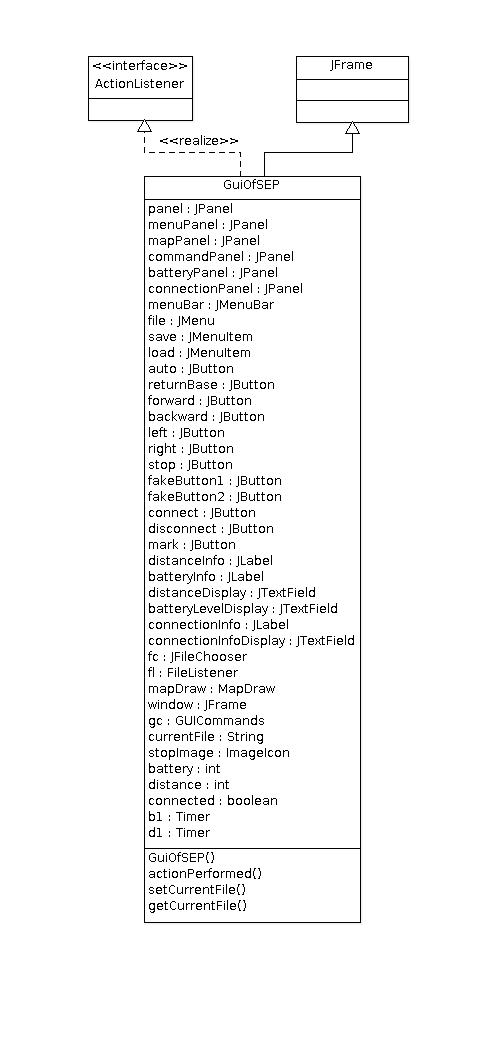
\includegraphics[width=10cm]{UML/GuiOfSEP.png}
\caption{The GuiOfSEP class diagram}
\label{Figure 2}
\end{figure}
     
\subsection{State Diagrams}

\begin{figure}[H]
\centering
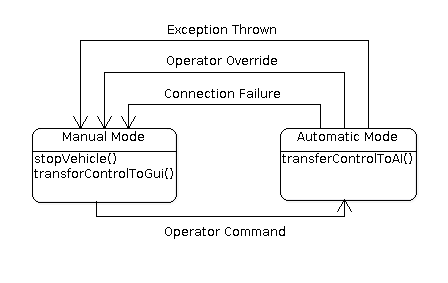
\includegraphics[width=10cm]{UML/ControllerFSM.png}
\caption{The ControllerFSM finite state machine diagram}
\label{Figure 3}
\end{figure}

\vspace{2cm}

\begin{figure}[H]
\centering
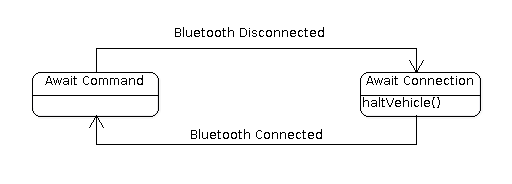
\includegraphics[width=12cm]{UML/RobotSideFSM.png}
\caption{The robot side finite state machine diagram}
\label{Figure 3}
\end{figure}
     
\begin{figure}[H]
\centering
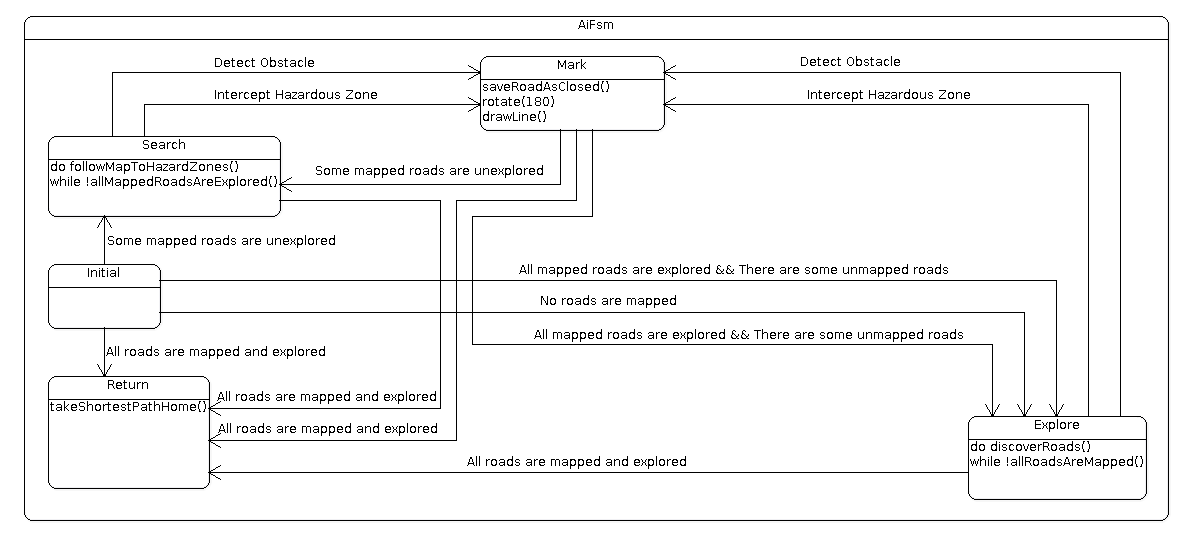
\includegraphics[width=19cm, angle=90]{UML/AiFsm.png}
\caption{The AiFsm finite state machine diagram}
\label{Figure 4}
\end{figure}

\section{Human Interface Design}

\subsection{Overview of the User Interface}

According to SRS, a GUI is essential on the PC side for the user to implement the following activities:

\begin{itemize}
\item The operator can establish communication with the robot by using GUI to manipulate the Bluetooth device.
\item The operator is able to manually control and monitor the robot's movement by operating a set of buttons and seeing a map panel.
\item The operator has the authority to command the robot to perform the AI mode by clicking buttons on the GUI, and then notice the robot status by receiving a bunch of messages showed on the GUI.
\item The operator is able to stop the movement of the robot by using the emergency stop button in the GUI whenever an emergency occurs.
\item The operator can control the robot in some perticular extents to ensure the optimised task completion of the robot through the GUI, e.g. monitoring the battery life or adjusting the speed of robot.
\end{itemize}

\noindent The design of the GUI is in accordance with SRS purposing a simulation of the real world to provide visibility of system status to user. The GUI should be consistent and standardised to ensure user control freedom, error provention, safety precaution, and risk handling. To achieve the ease of using for users, the GUI should be flexible, efficient of use, aesthetically friendly, minimalist design, and smooth for control flow. \\
\\
The development of the GUI follows the process below:

\begin{enumerate}
\item Relevant data gathering \\
Infer information for GUI from requirements; analyse user habits, contorl flow, and environments; derive from initial strategy and data presentation.
\item Prototypes \\
Create prototype based on the results of last phase.
\item Revisions \\
Show the prototype to stakeholders (the group and client) for feedbacks and recommendations. If passed move to next stage otherwise design a new prototype or modify the existed prototype.
\item Documentation \\
Create User Manual for the GUI.
\item Final review \\
Final demonstration for assessment.
\end{enumerate}

\subsection{Detailed Design of the User Interface}

According to the ``User Interface'' section of SRS, the GUI should consist of four parts:

\begin{enumerate}
\item Command buttons allow the operator to control the movement or change the status of the robot, including:
\begin{enumerate}
\item forward. Press once and the robot will continue moving forward.
\item backward. The same as forward.
\item left. Rotate the robot ninty degrees to left.
\item right. Rotate the robot ninty degrees to right.
\item connect. Establish the connection from PC to robot.
\item disconnect. Disconnect the bluetooth connection between PC and robot.
\item mark road closure. Command the robot to manually mark road closure.
\item start automatic mapping. Enable the AI mode of the robot to automatically explore the map.
\item return to base. Make the robot return to the starting position.
\item stop. The emergency stop for the robot.
\end{enumerate}
\item Robot information area contains the information in relation to the robot's status, including:
\begin{enumerate}
\item robot name.
\item battery level. Display the current battery level of the robot.
\item connection status. Display the status of Bluetooth connection using ``on'' and ``off''.
\item message. A textfield shows the messages sent by the robot including values of sensors, status of the robot, and warnings.
\end{enumerate}
\item Map area \\
A panel in the GUI to diaplay the current map. All objects defined in the DTD will be showed on the map, including roads, road intersections, obstacles, disaster area, closure, and unexplored area. The current location of the robot and traversed path by the robot would also be showed in the map.
\item List menu. \\
A menu that allows the operator to save and reload the map in the form of XML file in the format specified by the DTD by clicking items in the list menu.
\end{enumerate}

\noindent The display space for mapping is the major core component of the GUI, and it shall be maximised. All other functions except for the list menu are located at left-hand-side of the display window with a constant width so the display of map can be enlarged for larger screen sized window. The menu list is put on the top left of the window as a button on the top tool bar. The whole menu will emerge after a click on the menu button. Inside the menu list the user will see menu items to deal with the XML file. \\
\\
The functions of GUI, which were designed upon the requirements elicitation, are outlined as following:

\begin{enumerate}
\item R01 and H02: Manual Control of the robot: \\

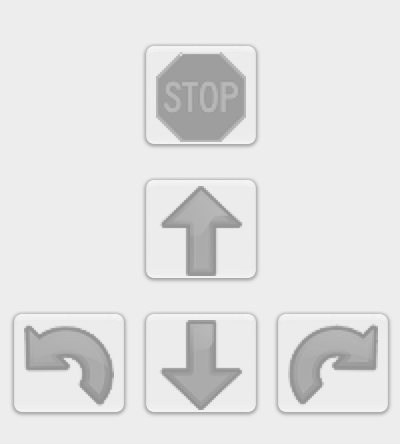
\includegraphics[width=11.5cm]{images/movement.png}
\vspace{15pt}

\item R02-03: Map saving and loading: \\

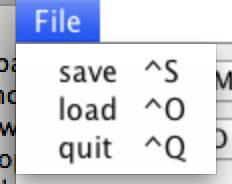
\includegraphics{images/menu.png}
\vspace{15pt}

\item R07: Road closure marking: \\


\includegraphics{images/closure.png}
\vspace{15pt}

%\newpage
\item H01: The whole GUI: \\

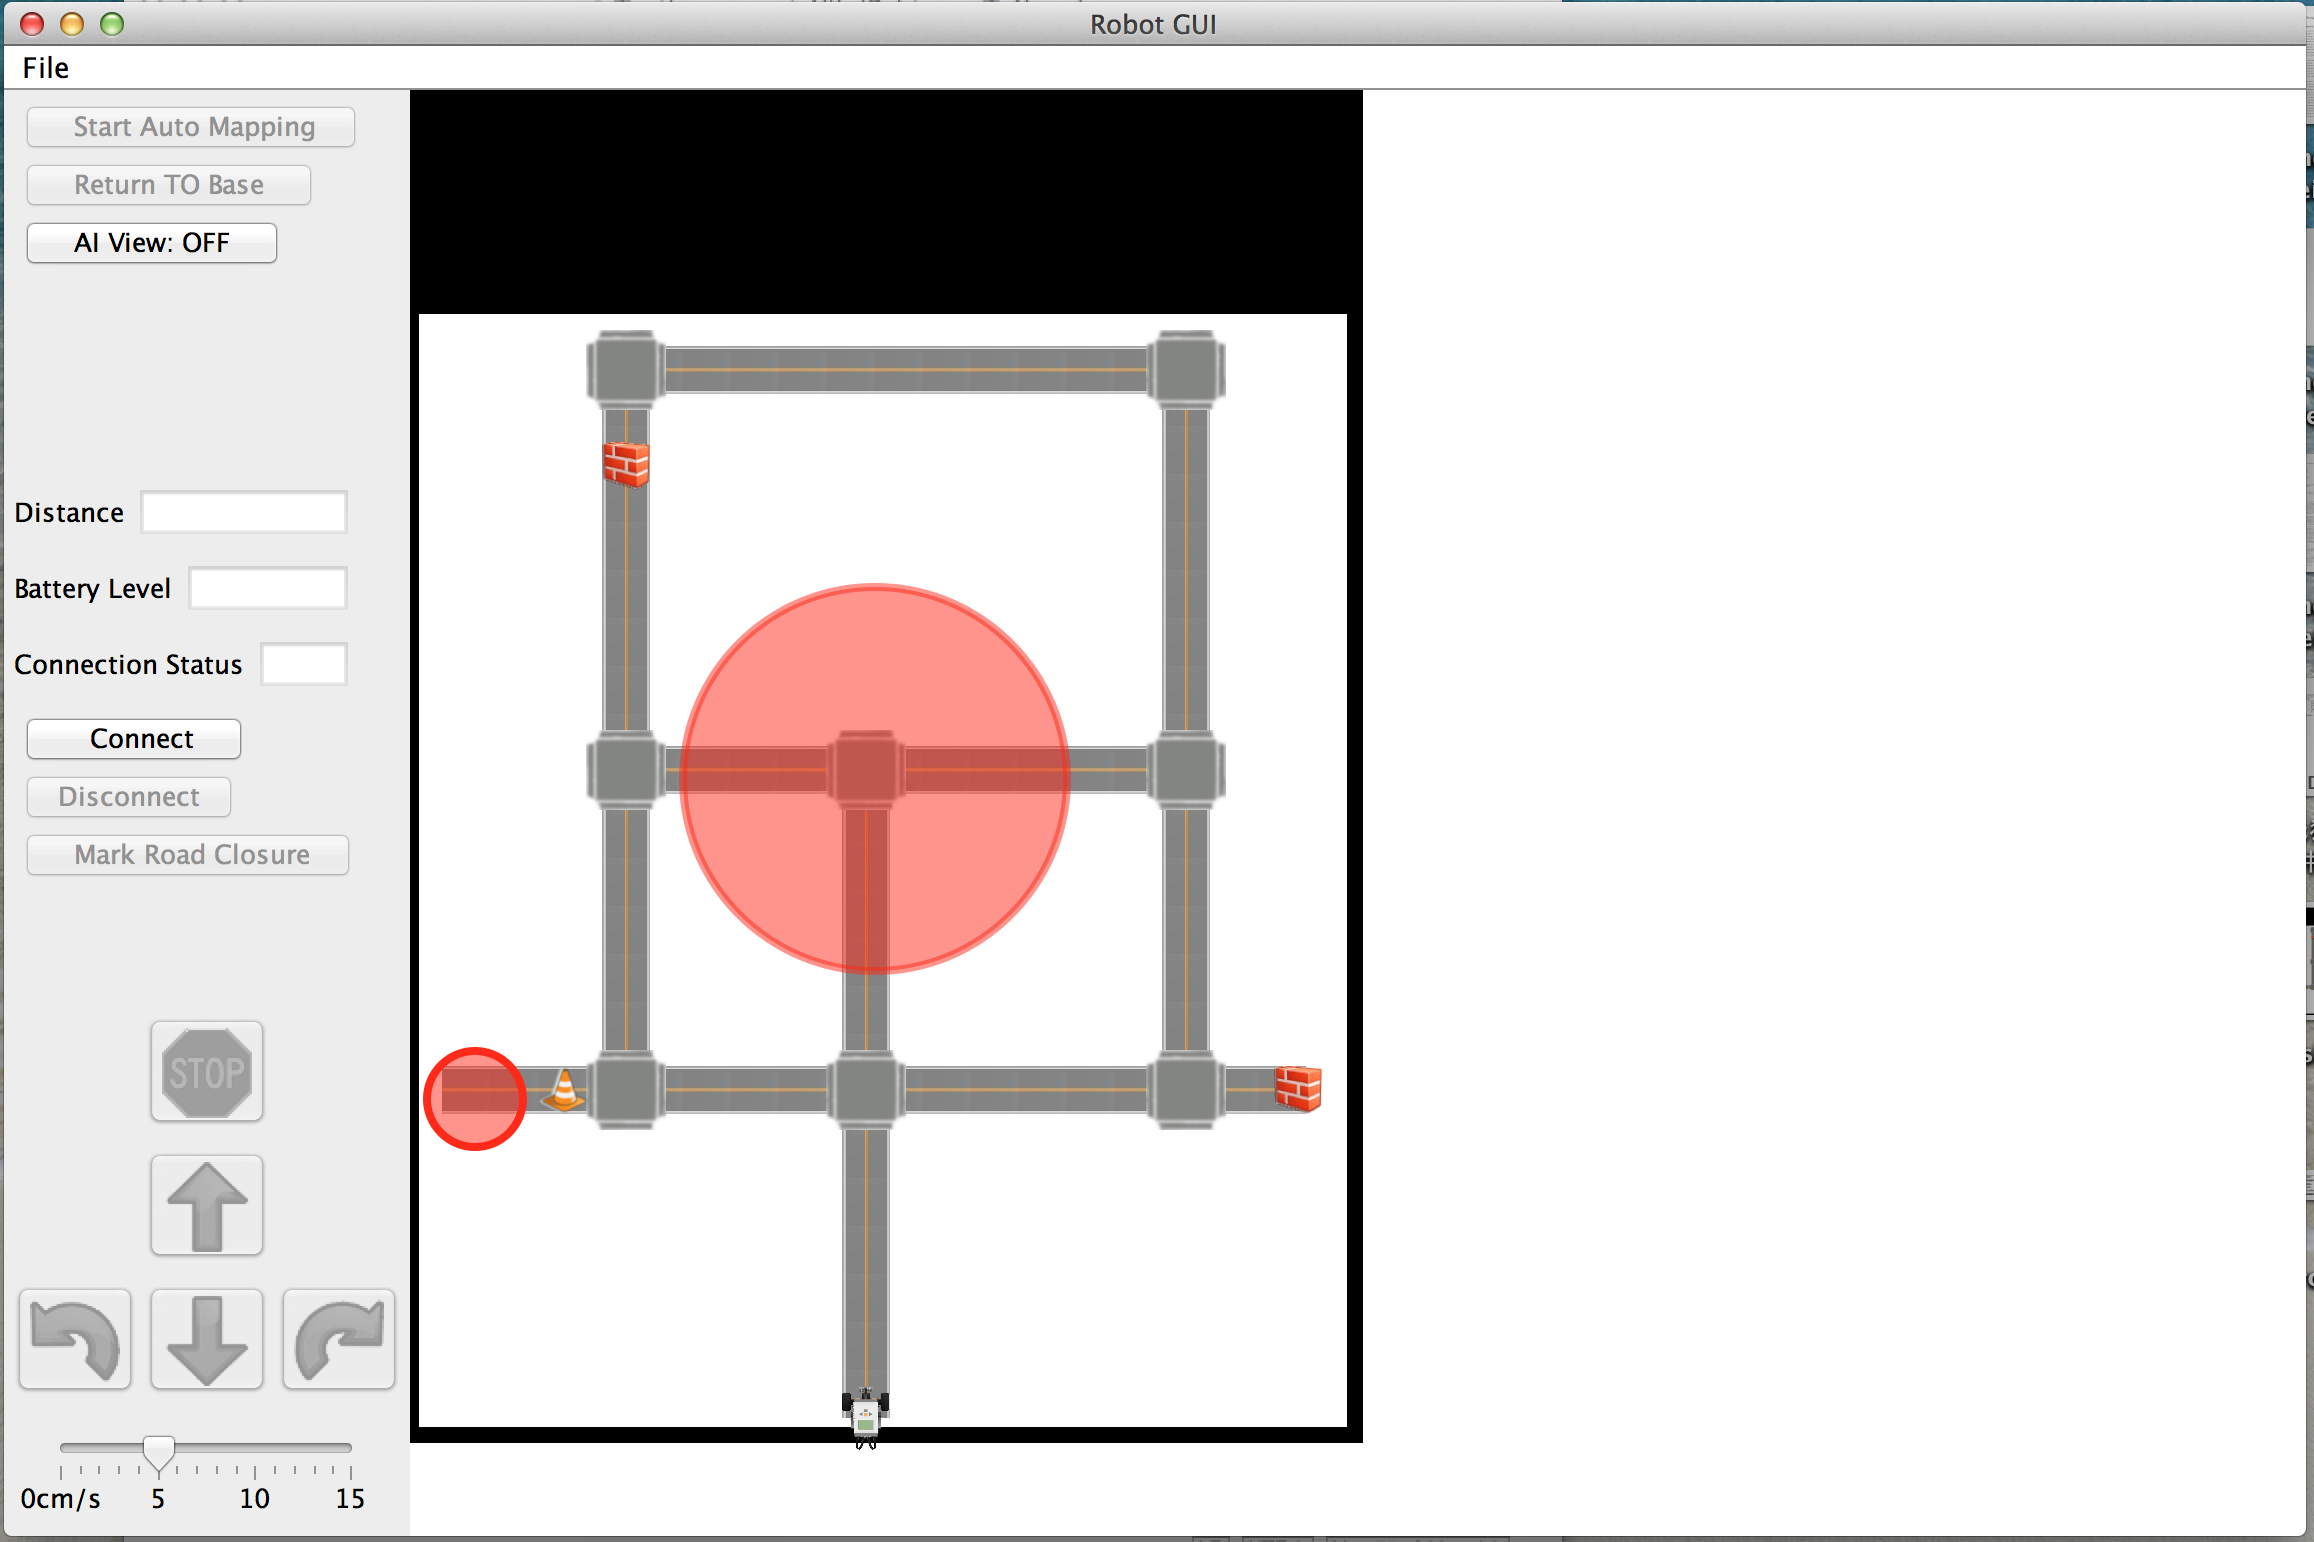
\includegraphics[width=11.5cm]{images/whole.png}
\vspace{15pt}

\item H04: Emergency stop: \\


\includegraphics{images/stop.png}
\vspace{15pt}

\item Other attributes stated in other descriptions of SRS: \\
\\
AI mode: \\

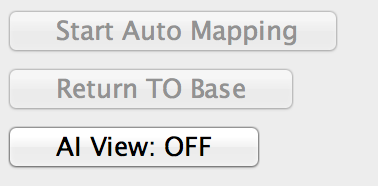
\includegraphics{images/AI.png}
\vspace{15pt}
\\
\\

Status: \\

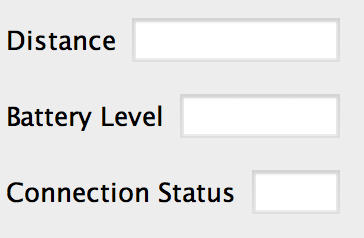
\includegraphics{images/status.png}
\vspace{15pt}

Connection: \\


\includegraphics{images/connect.png}
\vspace{15pt}

\newpage
\item The display of the map: \\

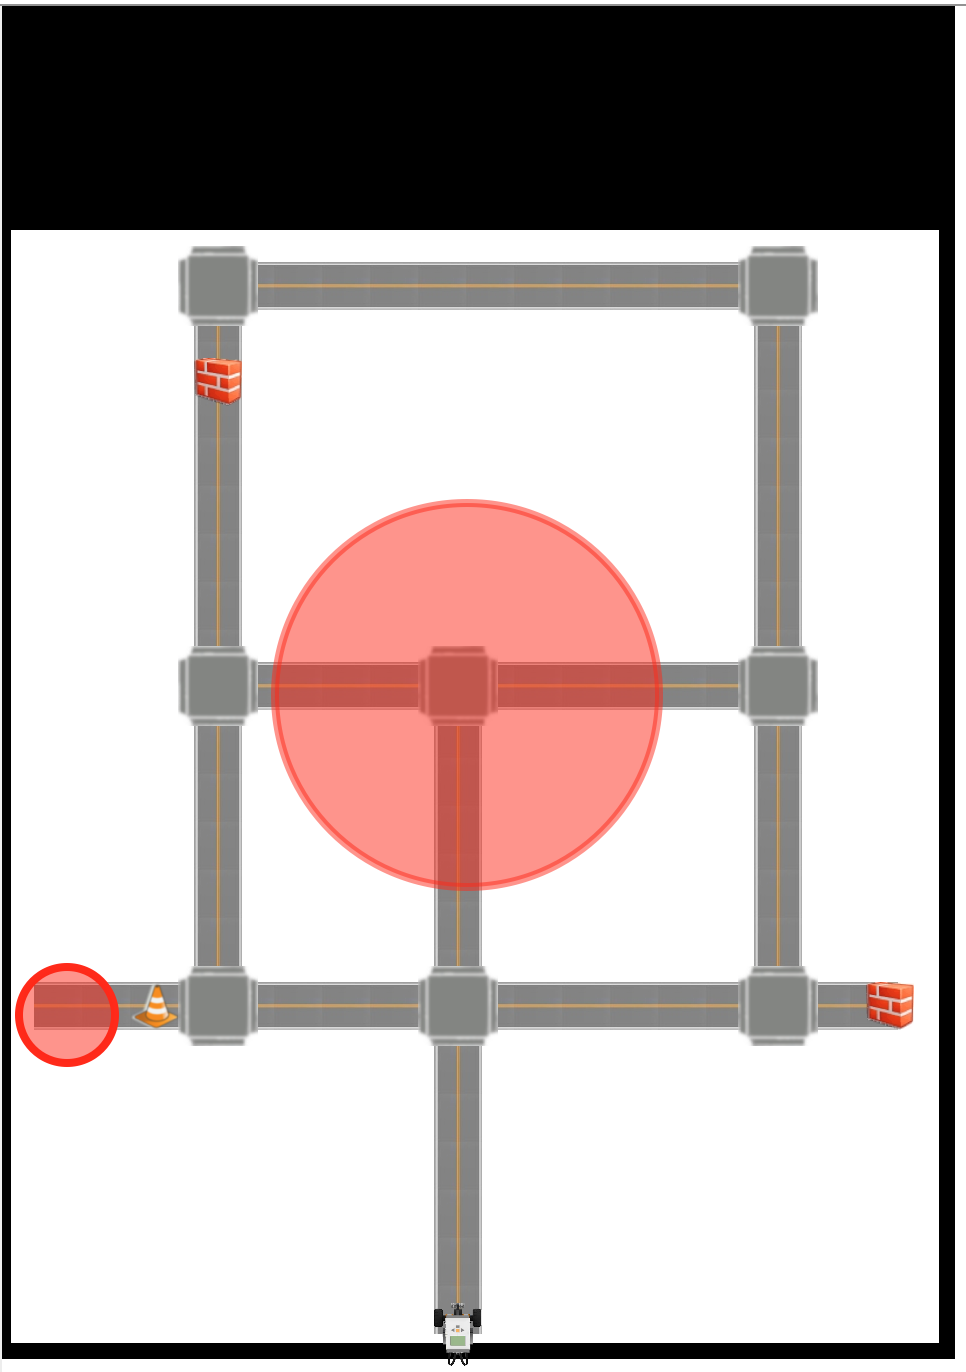
\includegraphics{images/map.png}
\vspace{15pt}
\end{enumerate}

\noindent The functions that have already been defined in SRS but not been implemented yet in the GUI, are outlined as following:

\begin{enumerate}
\item M01: Display the taversed path by the robot in map panel.
\item H03: Display the current position of robot in map panel.
\item H06: A textfield on the GUI to show messages such as alert message.
\item SA01: A speed bar on the GUI to adjust the speed of the robot. The speed should be within a safe speed.
\item Other function that was not described in SRS: Zoom feature for the map.
\end{enumerate}
    
\newpage

\section{Resource Estimates}

The minimum hardware requirements are: Intel Pentium Dual-Core CPU E5200 with clock rate of 2.50G HZ; 3.7 GB Memory and 128GB Hard-disk Space. \\

\newpage

\section{Definitions, Acronymns and Abbreviations}

%%Acronym Definitions
%%(ref: http://ctan.unsw.edu.au/macros/latex/contrib/acronym/acronym.pdf)

\begin{acronym} 
\acro{api}[API]{Application Programming Interface}
\acro{cp}[Coding Pharaohs]{The software developing team undertaking the project} 
\acro{dtd}[DTD]{Document Type Definition}
\acro{gui}[GUI]{Graphical User Interface}
\acro{jvm}[JVM]{Java Virtual Machine}
\acro{pin}[PIN] {Personal Identification Number}
\acro{rcmr}[RCMR] {Road Closure Marking Robot}
\acro{sdd}[SDD]{Software Design Document}
\acro{sep}[SEP]{Software Engineering and Project}
\acro{spmp}[SPMP]{Software Project Management Plan}
\acro{srs}[SRS]{Software Requirements Specification}
\acro{svn}[SVN]{Subversion}
\acro{tbd}[TBD]{To Be Determined}
\acro{xml}[XML]{Extensible Markup Language} used to store map information

\end{acronym}
  
\end{document}
